 \chapter{Frequency comb generation through active modulation of a continuous-wave laser}\label{chap:EOMCombs}
   \begin{footnotesize}
 	\begin{spacing}{1.2}
 		This chapter describes work that was reported in:
 		\begin{itemize}
 			\item \fullcite{Cole2016}.\\
 			\item \fullcite{Beha2017}.\\
 		\end{itemize}
 	\end{spacing}
 \end{footnotesize}

This chapter discusses the generation of high repetition-rate frequency combs through electro-optic modulation of a continuous-wave laser---so-called EOM combs \cite{Kobayashi1972,Kourogi1993,Murata2000,Sakamoto2007,Morohashi2008,Ishizawa2010,Wu2010,Supradeepa2012,Metcalf2013,Wu2013}. This scheme represents an alternative to parametric generation of high repetition-rate combs in Kerr resonators, and as the technology matures it will likely find a niche in the application space that leverages its long-term stability, lack of moving parts, and possibility for robust turn-key operation. First we present the operational principle of the EOM comb, followed by experimental results that represent the first $f-2f$ self-referencing of a comb of this kind. Then we discuss noise processes that are specific to the EOM comb, the investigation and mitigation of which is a significant contribution of the work described here. A proof-of-principle application of the EOM comb to the generation of low-noise microwave is presented, and the chapter concludes with a brief outlook for the technology.

\section{Principle of operation}
At its simplest, an EOM comb is a set of lines generated by passing a CW `seed' laser through cascaded phase and intensity modulators to generate a train of chirped pulses. After this initial step, the pulse train may be propagated through a dispersive medium to temporally compress the pulses, and they can be subsequently spectrally broadened. A generic expression for the electric field before temporal compression results from the product of the carrier field $E_oe^{i\omega_ct}$ with operators $\cos\Phi(t)$ representing the intensity modulation and $\mathrm{exp}\left[i\delta_{PM} \sin{\omega_{rep} t}\right]$ representing the phase modulation. Here $E_o$ and $\omega_c$ are the complex amplitude and the carrier frequency of the seed laser. The intensity modulation profile is:
\begin{equation}
\Phi(t)=\phi_{DC}+\phi_{RF}\sin{(\omega_{rep}t+\phi_{IMPM})}.
\end{equation}
The phases $\phi_{DC}$ and $\phi_{RF}$ represent the DC bias and depth of the intensity modulation, respectively, which experimentally are sourced from a DC power supply and an RF synthesizer. The phase-modulation index, which sets the initial bandwidth of the EOM comb, is $\delta_{PM}$. The comb's repetition rate is $f_{rep}=\omega_{rep}/2\pi$, with $\omega_{rep}$ the angular frequency of the phase and intensity modulation. In practice it is useful to derive these signals from the same synthesizer. The phase $\phi_{IMPM}$ represents a phase difference between the IM and PM operators arising from path-length differences, which can be controlled via the insertion of a phase shifter in one electrical path. 

\begin{figure}[htpb]
	\begin{center}
		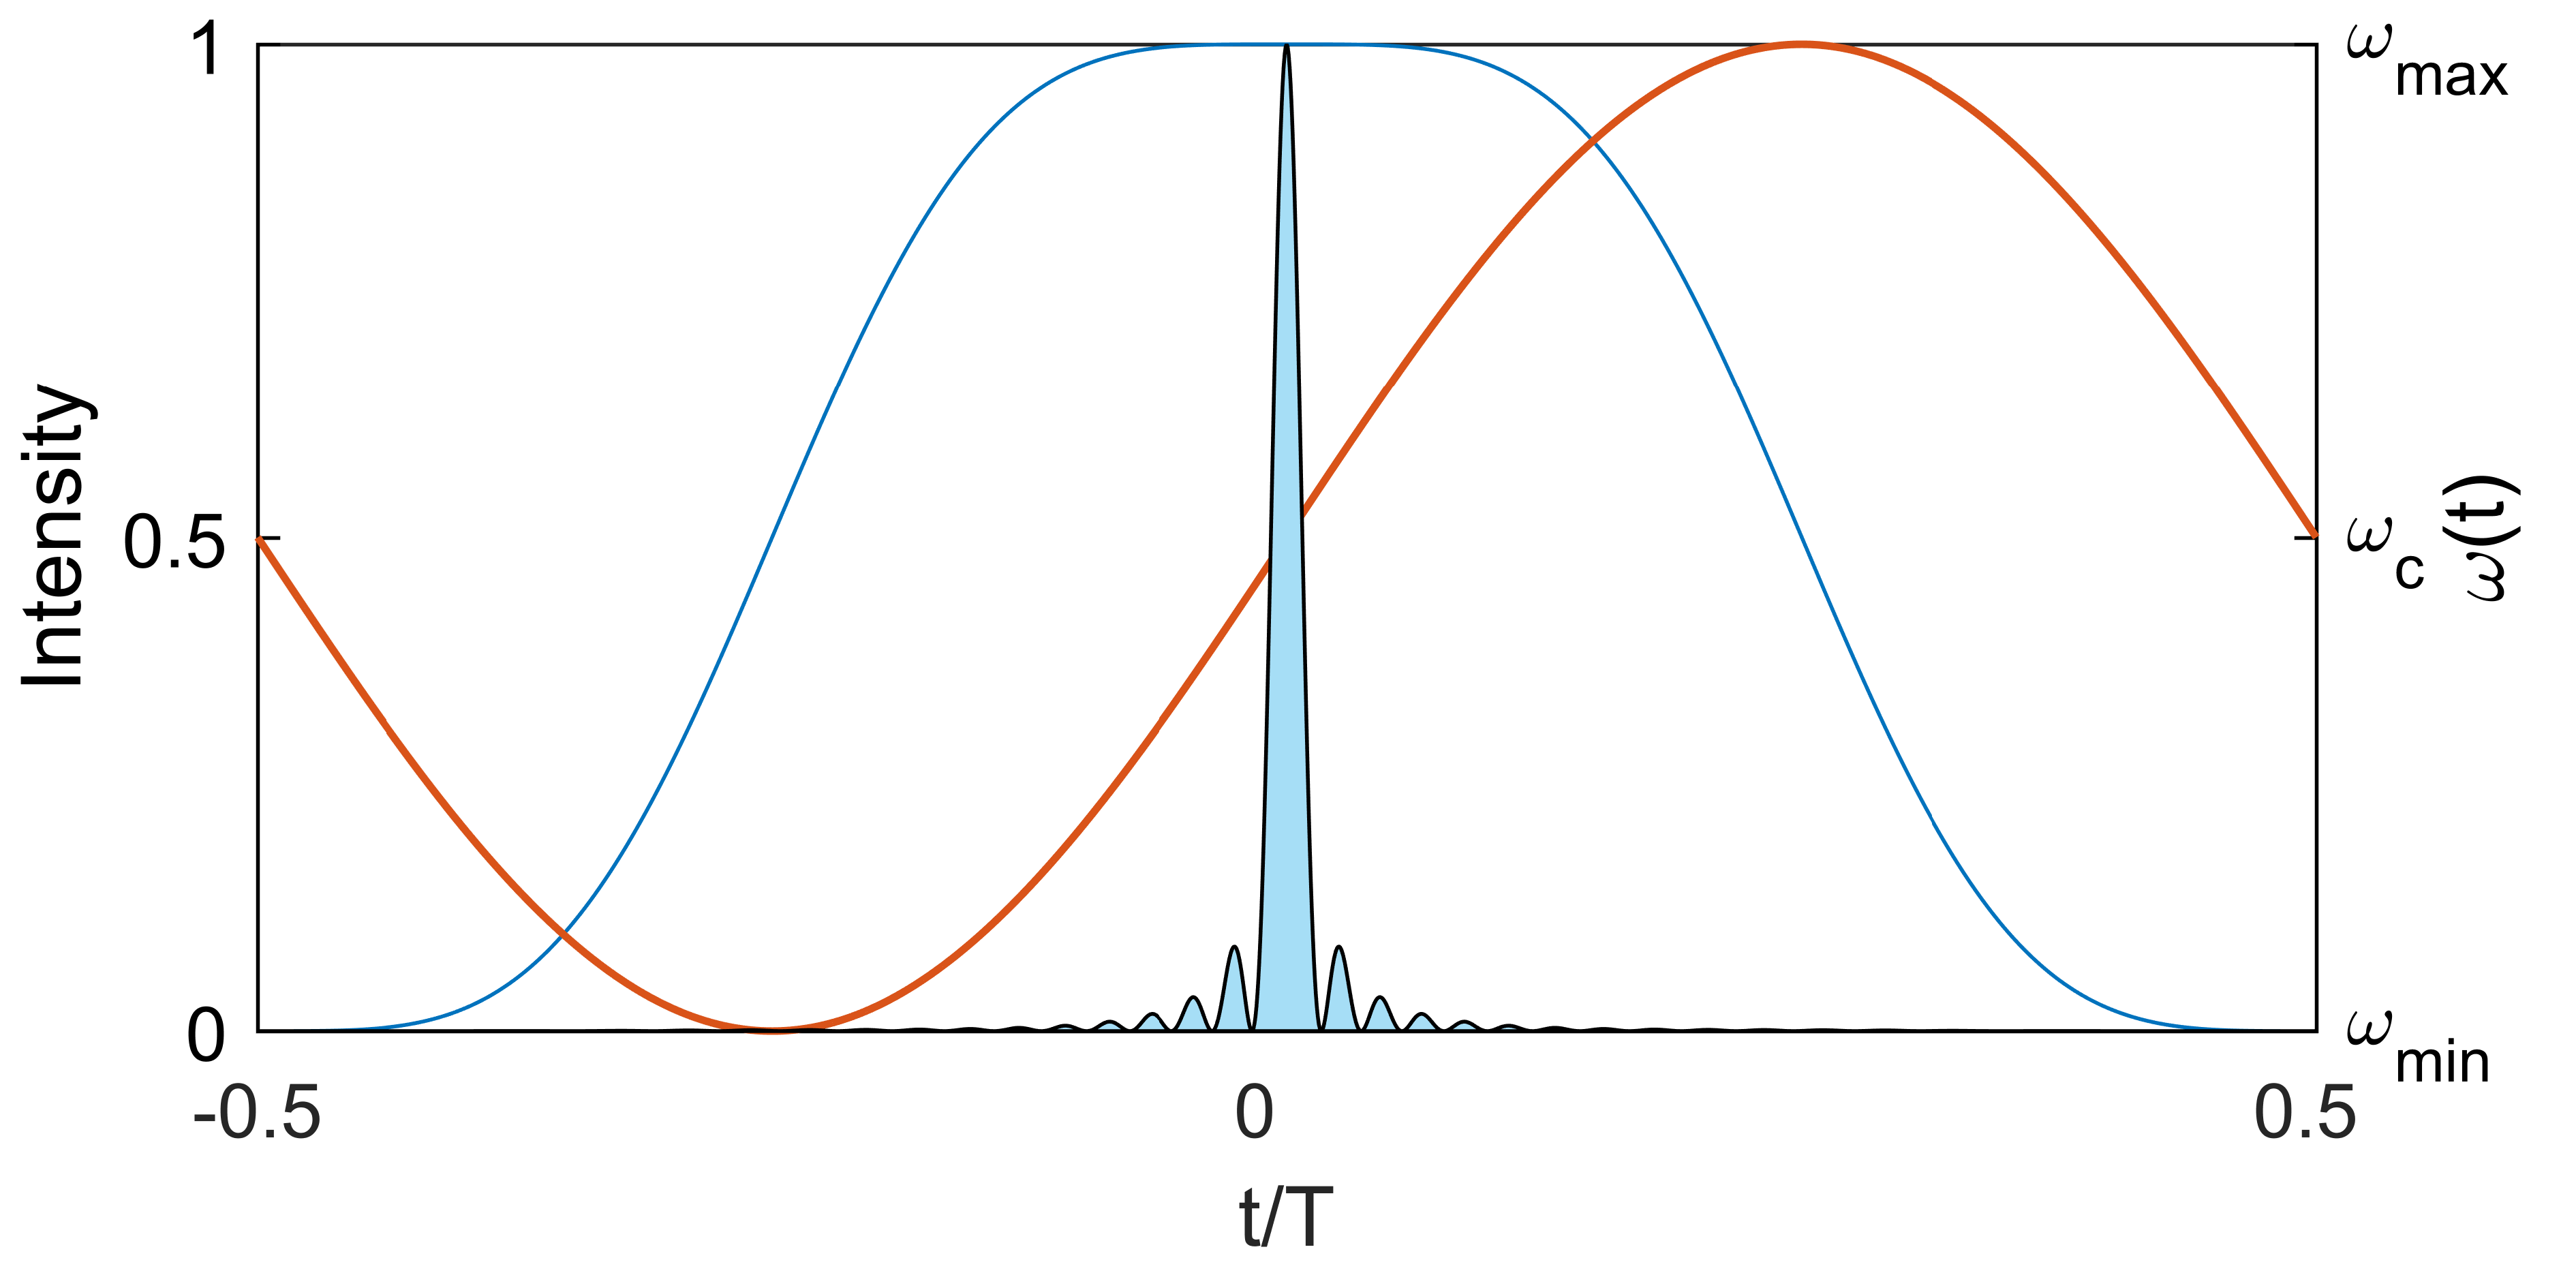
\includegraphics[]{\FigPath/Figures/EOMCombs/EOMCconcept.png}
	\end{center}
	\caption[Operating principle of an electro-optic modulation comb]{\textbf{Operating principle of an electro-optic modulation comb.} A train of chirped pulses is generated by combined electro-optic phase and intensity modulation,  and the pulses can then be conveniently temporally compressed in a dispersive medium. Light blue line (plotted with respect to the left axis): Initial intensity profile of a single EOM comb pulse as described by Eq. \ref{eq:EOMC}. Orange (right axis): Instantaneous carrier frequency, which varies about $\omega_c$ by $\pm\delta_{PM}\omega_{rep}$ and increases approximately linearly in time while the pulse amplitude is high. Solid blue (left axis): Pulse resulting from compression of the initial pulse to its transform limit. The temporal duration of this pulse decreases as $\delta_{PM}$ increases as a result of the increased bandwidth of the comb; here the phase-modulation depth $\delta_{PM}=31\pi/4$ is used. The compressed pulse has higher peak power (in this case by a factor of 26.5); for convenient depiction of both pulses the compressed pulse has been rescaled.}
	\label{fig:EOMCconcept}
\end{figure} 

For convenient temporal pulse compression and subsequent spectral broadening of the comb it is desirable to configure the IM and PM to yield a train of 50 $\%$ duty-cycle pulses with normal chirp (temporally increasing carrier frequency). To achieve this, both $\phi_{DC}$ and $\phi_{RF}$ are set to $\pi/4$ and $\phi_{IMPM}$ is set to zero. Experimentally, one can determine the appropriate RF drive power and bias by adjusting the ratios $\eta_1=P_1/P_0$ and $\eta_2=P_2/P_0$ between the first- and second-order sidebands and the carrier to $\eta_1=-7.4$ dB and $\eta_2=-21.3$ dB with only intensity modulation applied to the seed laser.\footnote{This assumes that the modulation is applied to both paths in the intensity modulator with opposite sign; the correct ratios for a Mach-Zehnder intensity modulator with modulation in only one path are $\eta_1=-5.8$ dB and $\eta_2=-12.9$ dB. This difference arises from residual phase modulation on the output field in the latter case. To determine the internal configuration of the modulator, one can examine the action of the bias: if the modulation is applied to both paths with opposite signs, the bias will adjust only the ratios between the odd- and even-order sidebands while leaving the ratios within each group fixed. However, if the modulation is applied to only one path, the bias will change the ratio of each sideband to the carrier. These conclusions are reached by application of various forms of the Jacobi-Anger expansion.} Setting $\phi_{IMPM}$ to either zero or $\pi$ is achieved by examining the optical spectrum of the EOM comb with both IM and PM applied. The spectrum is asymmetric if $\phi_{IMPM}$ is not zero or $\pi$ due to stronger transmission of either the high- or low-frequency components of the phase-modulated seed laser through the intensity modulators. The optical spectrum of the comb, which does not include phase information, is the same for $\phi_{IMPM}=0$ or $\pi$; the difference between the two corresponds to reversal of the field in time or, equivalently, the difference between normal and anomalous chirp. Setting $\phi_{IMPM}$ to zero is accomplished by verifying that the pulses are compressed by propagation in an appropriate length of an anomalously dispersive medium; $\phi_{IMPM}=\pi$ corresponds to anomalous chirp on the initial pulse train, in which case the pulses will not be compressed.

A simplified and illuminating expression for the electric field of a normally-chirped 50 $\%$ duty-cycle pulse train (up to a constant overall phase shift relative to the expressions above) is:
\begin{equation}
E=E_o\cos\left(\frac{\pi}{2}\sin^2{\frac{\omega_{rep}t}{2}}\right)e^{i\omega_ct-i\delta_{PM}\cos{\omega_{rep}t}}. \label{eq:EOMC}
\end{equation}
This can be understood as the product of a time-varying real amplitude $a(t)=E_o\cos\left(\frac{\pi}{2}\sin^2{\frac{\omega_{rep}t}{2}}\right)$ and a phase factor from which the instantaneous carrier frequency $\omega(t)=\omega_c+\omega_{rep}\delta_{PM}\sin{\omega_{rep}t}$ can be calculated. The carrier frequency $\omega(t)$ is increasing when the amplitude $a(t)$ is at its maximum, corresponding to normal chirp on the pulses. Fig. \ref{fig:EOMCconcept} depicts the intensity $|E|^2$ and instantaneous carrier frequency of the field given by Eq. \ref{eq:EOMC}, as well as the intensity profile corresponding to compression of the same spectrum to its transform limit.




\section{Generation of an EOM comb and detection of its carrier-envelope offset frequency}

This section describes the generation of an EOM comb with 10 GHz repetition rate and subsequent measurement of its carrier-envelope offset frequency. One advantage of the EOM comb scheme is that the generation and spectral broadening of the comb is well understood, and can be modeled accurately. To demonstrate this, the results of simulations of the comb and the experimental output are compared at each stage in the generation process.

The experimental setup is depicted in Fig. \ref{fig:EOMC_Schematic}. The basic experimental scheme consists of the following steps: 1. Initial generation and temporal compression of the EOM comb pulse train; 2. Modest spectral broadening and temporal re-compression, along with propagation through a Fabry-Perot filter cavity for noise reduction (see Sec. \ref{sec:EOMCnoise}); and 3. Octave-spanning supercontinuum generation and detection of the carrier-envelope offset frequency. The results described below represent the first time a frequency comb of this kind has been self-referenced. Key to the success of this approach is the implementation of nonlinear spectral broadening in two stages, which allows the second stage to be seeded with $\sim$130 fs pulses for coherent supercontinuum generation. Noise reduction with the Fabry-Perot filter cavity is also critical for coherent spectral broadening; this is described in detail in Sec. \ref{sec:EOMCnoise}.

To generate the initial train of chirped pulses, a telecommunications-band CW laser is passed through cascaded phase and intensity modulators driven with a 10 GHz microwave signal. The intensity modulator is biased at the 50 \% transmission point and driven with an RF amplitude appropriate for generation of a 50 $\%$ duty-cycle pulse train, as described above;  the phase modulator is driven with modulation depth of $\sim31\pi/4\sim24.3$ rad. The relative phase between the modulators is set such that the phase applied by the phase modulator is at a minimum when the transmission of the intensity modulator is highest; this yields a train of normally-chirped (up-chirped) pulses. Fig. \ref{fig:EOMC_Schematic}, Panel (i) presents a comparison between the simulated and measured spectra for the initial pulse train. 


\begin{figure}[htpb]
	\begin{center}
		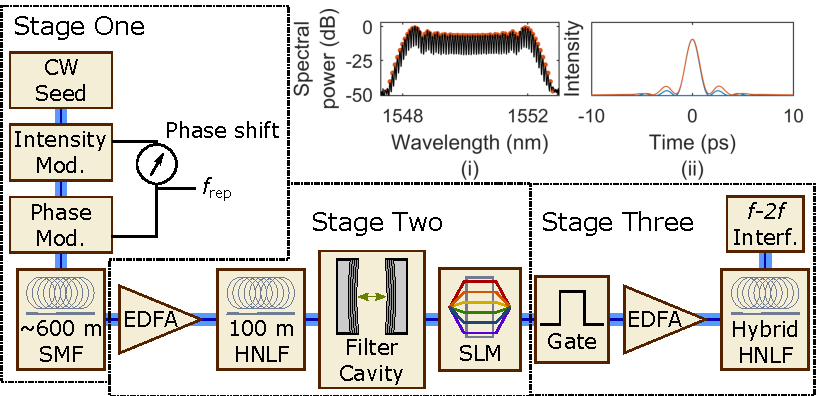
\includegraphics[]{\FigPath/Figures/EOMCombs/EOMCsetup.pdf}
	\end{center}
	\caption[Experimental setup for detection of the carrier-envelope offset frequency of an EOM comb after generation of a coherent supercontinuum]{\textbf{Experimental setup for detection of the carrier-envelope offset frequency of an EOM comb after generation of a coherent supercontinuum.} Detection of $f_0$ is performed with a three stage experiment. In Stage 1 a train of $\sim$1.5 ps pulses is generated. In Stage 2 these pulses are spectrally broadened and temporally compressed to $\sim$130 fs duration. In Stage 3 an octave-spanning supercontinuum is generated and $f_0$ is detected in an $f-2f$ interferometer. Panel (i) shows the measured spectrum of the comb output by Stage 1 (black), along with a simulation of the same (orange). Panel (ii) shows simulation of the temporal compression of the pulses by propagation in 570 m of single-mode fiber (orange) and to the transform limit (blue).}
	\label{fig:EOMC_Schematic}
\end{figure} 


Next, the chirped pulse train is propagated through 600 m of anomalously-dispersive SMF. The length of SMF that is appropriate for pulse compression depends on the bandwidth of the optical pulses to be compressed; equivalently, it depends on both the phase-modulation depth and the repetition rate of the pulse train. This temporal compression reduces the duration of the optical pulses from $\sim$50 ps to $\sim$1.5 ps. A simulation of the resulting intensity profile and a comparison to the spectrum's transform-limited pulse profile is presented in Fig. \ref{fig:EOMC_Schematic}, Panel (ii). 

The compressed pulses are amplified to 400 mW average power in an erbium-doped fiber amplifier and launched into 100 m of HNLF. This section of HNLF has chromatic dispersion that is small and normal; this is carefully chosen to chirp the pulses via self-phase modulation while avoiding soliton-fission dynamics \cite{Dudley2006}. The result is a train of chirped $\sim$1.5 ps pulses exiting the fiber.  In Fig. \ref{fig:EOMC_Broadening}a we present the measured optical spectrum of this pulse train, as well as results of a numerical simulation of the spectral broadening in the 100 m of normally-dispersive HNLF. These simulations are conducted using the nonlinear Schrodinger equation (NLSE) including third order dispersion \cite{Agrawal2007}, taking as initial conditions the calculated SMF-compressed intensity profile of the EOM comb pulses shown in Fig. \ref{fig:EOMC_Schematic}(ii). The dispersion values for the HNLF used in the simulation are $D=-0.04$  ps/nm$\cdot$km and $D'=0.003$ ps/nm$^2\cdot$km, close to the values specified by the manufacturer. The simulation method is described in detail in Appendix \ref{app:numericalsims}.

%\begin{figure}[htpb]
%	\begin{center}
%		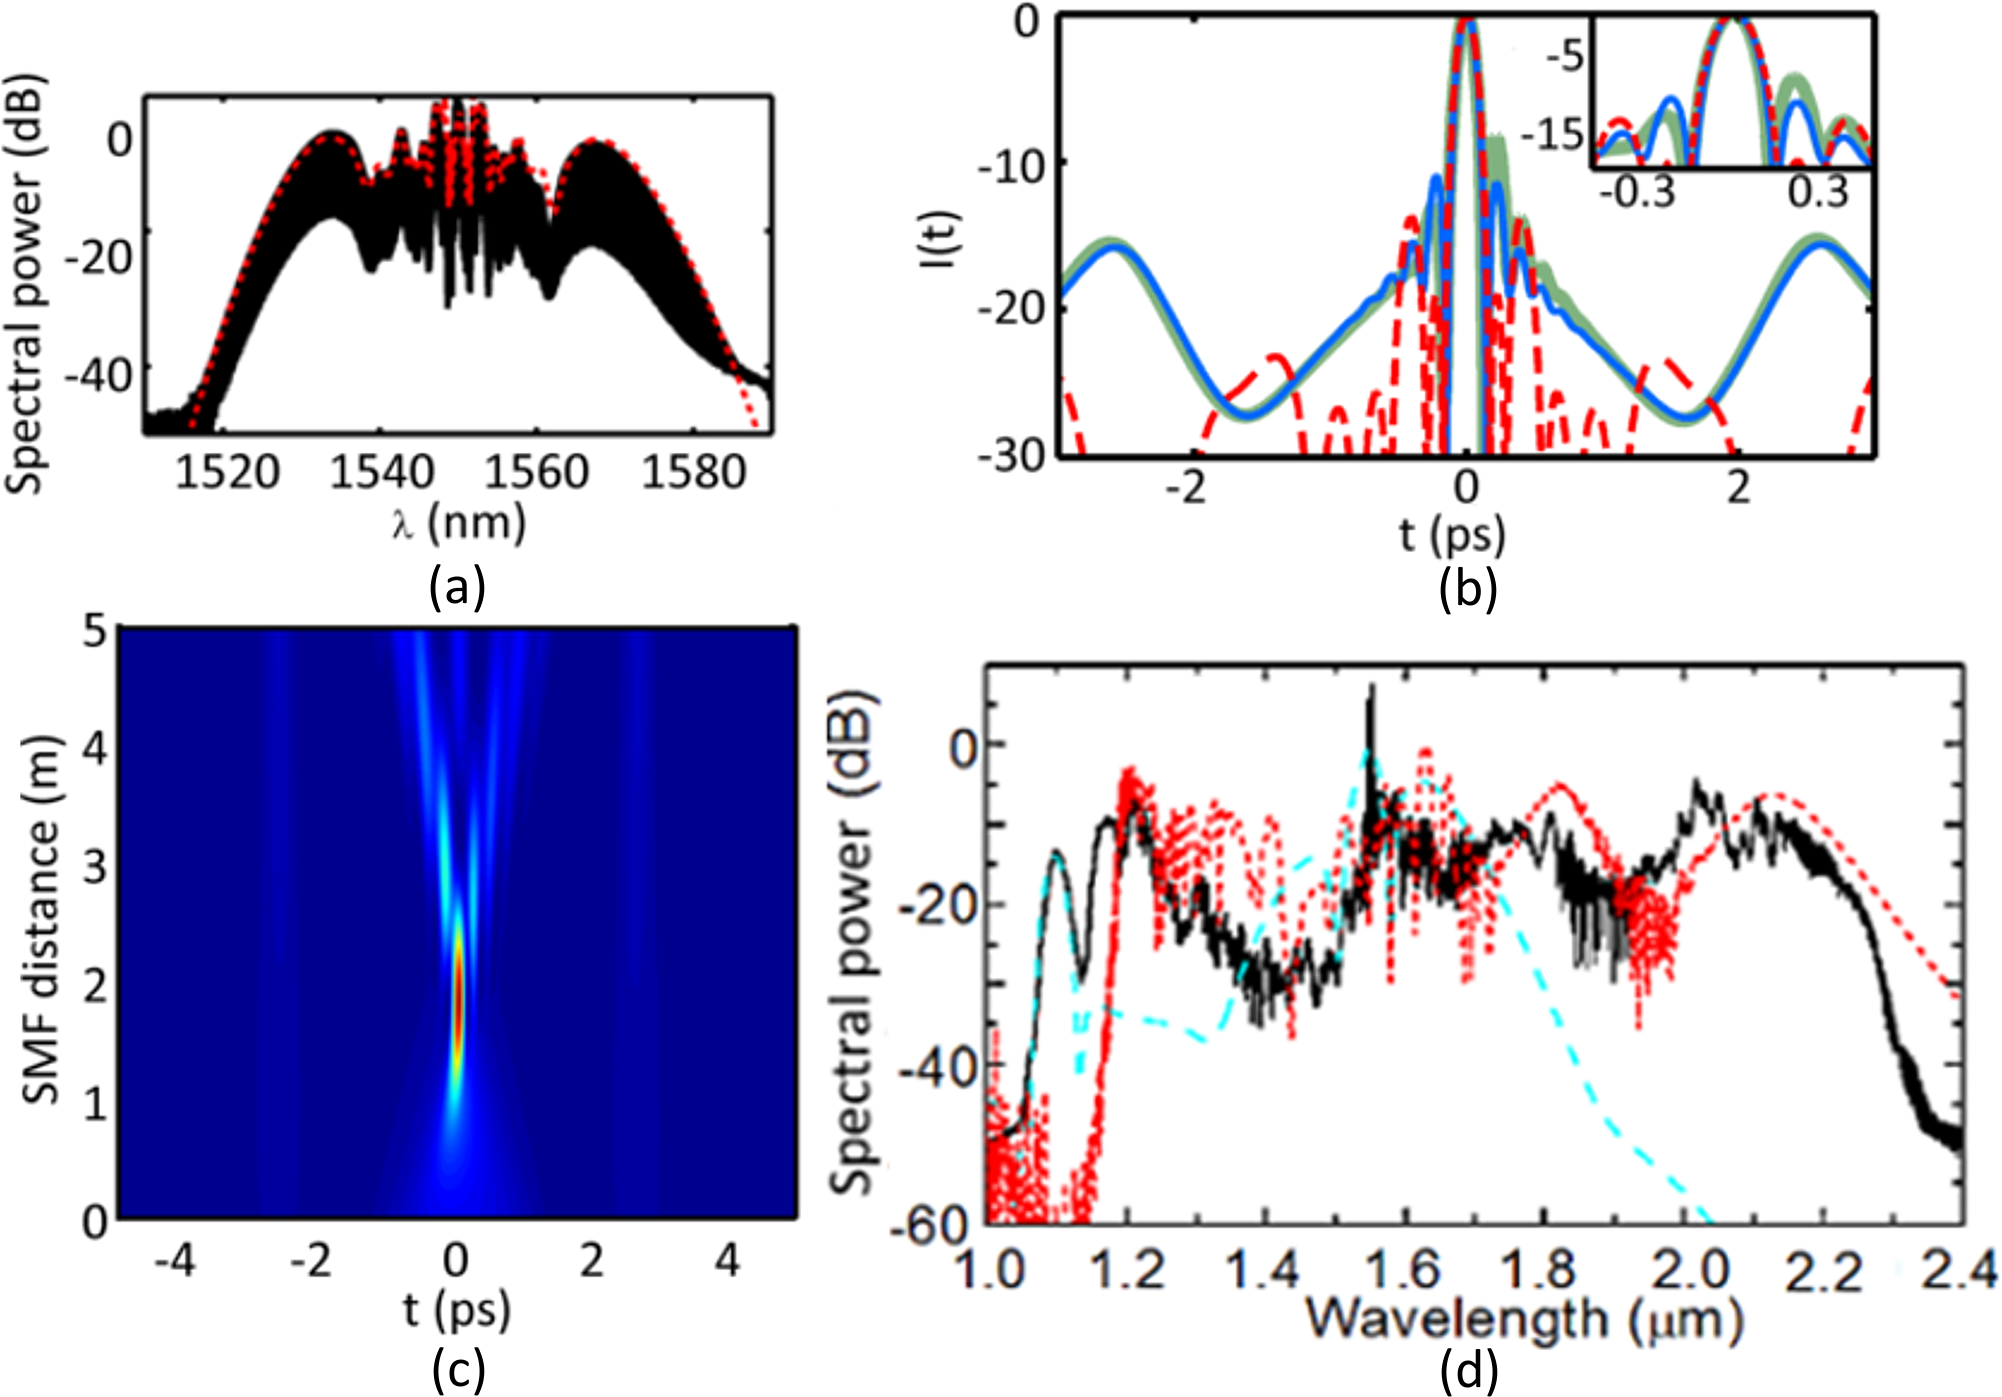
\includegraphics{\FigPath/Figures/EOMCombs/EOMC_spectraWsims.png}
%	\end{center}
%	\caption[Figure Title]{\textbf{Spectral broadening for generation of an octave-spanning supercontinuum.} (a) Measured optical spectrum after propagation in 100 m of low-normal-dispersion HNLF (black). The spectrum is broadened by self-phase modulation, which imposes a chirp on the pulses. Shown in red is a simulation of the same, conducted as described in the text. (b) Logarithmic-scale plot of the simulated pulse intensity envelopes after temporal recompression in the SLM with 2\textsuperscript{nd}-, 3\textsuperscript{rd}-, and 4\textsuperscript{th}-order dispersion (blue), in an appropriate length of SMF (thick green), to the transform limit (dashed red). (c) Simulated re-compression of the SPM-chirped pulses (red spectrum in panel (a)) in SMF. (d) Measured optical spectrum of the octave-spanning supercontinuum generated by the EOM comb system (black), plotted along with simulated spectra calculated as described in the text to investigate the effects of the 30 cm, highly-dispersive piece of HNLF (long-dashed teal) and the 7.7 m, lower-dispersion piece of HNLF (short-dashed red).}
%	\label{fig:EOMC_Broadening}
%\end{figure} 



\begin{figure}[htpb]
	\begin{center}
		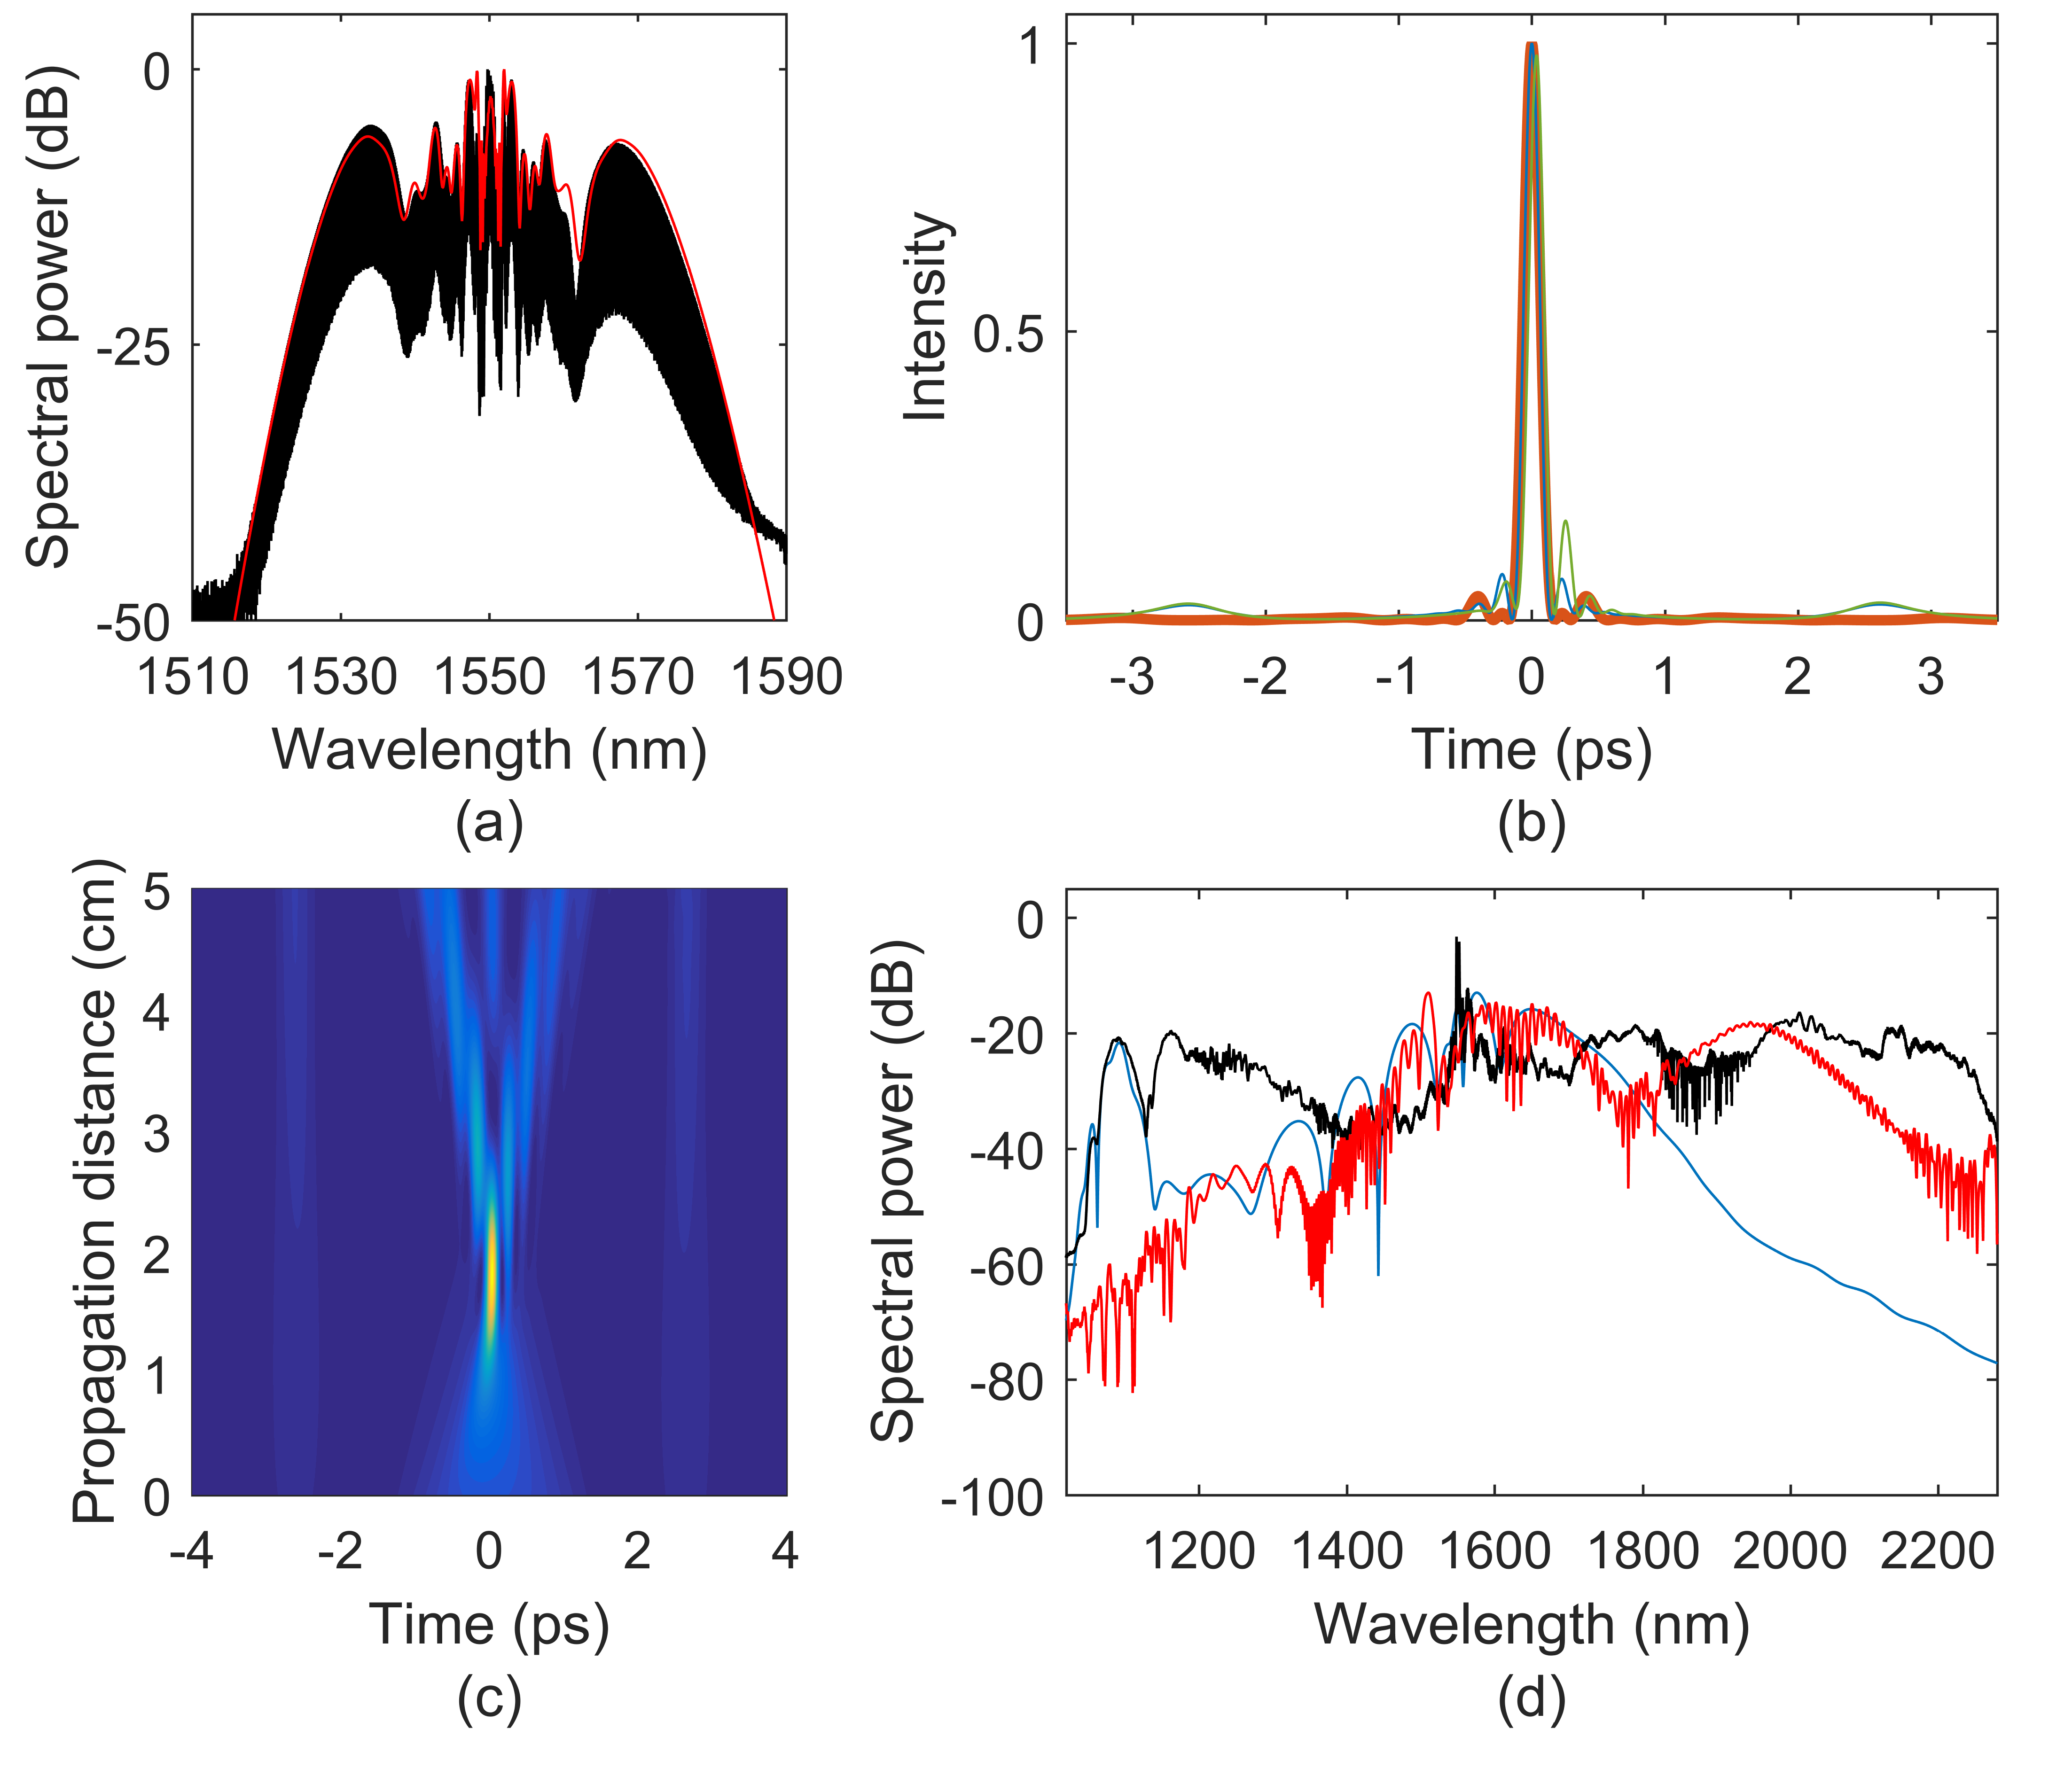
\includegraphics{\FigPath/Figures/EOMCombs/EOMC_spectraWsimsv3_diffcolor.png}
	\end{center}
	\caption[Spectral broadening for generation of an octave-spanning supercontinuum]{\textbf{Spectral broadening for generation of an octave-spanning supercontinuum.} (a) Measured optical spectrum after propagation in 100 m of low-normal-dispersion HNLF (black). The spectrum is broadened by self-phase modulation, which imposes a chirp on the pulses. Shown in red is a simulation of the same, conducted as described in the text. (b) Simulated pulse intensity envelopes after temporal re-compression to the transform limit (thick orange), in the SLM with 2\textsuperscript{nd}-, 3\textsuperscript{rd}-, and 4\textsuperscript{th}-order dispersion (blue), and in an appropriate length of SMF (green). FWHM pulse durations are similar, but the SLM- and SMF-compressed pulses have energy in satellite pulses at $\pm$2.5 s, and the SMF-compressed pulse has a significant asymmetry. (c) False-color plot of simulated re-compression of the SPM-chirped pulses (red spectrum in panel (a)) in SMF. A minimum pulse duration of $\sim$140 fs is achieved after propagating through 1.93 cm of SMF. (d) Measured optical spectrum of the octave-spanning supercontinuum generated by the EOM comb system (black), plotted along with simulated spectra calculated as described in the text to investigate the effects of the 30 cm, highly-dispersive piece of HNLF (blue) and the 7.7 m, lower-dispersion piece of HNLF (red).}
	\label{fig:EOMC_Broadening}
\end{figure} 

After propagation through the first section of HNLF, the pulses are passed through a high-finesse Fabry-Perot cavity for suppression of optical frequency fluctuations as discussed below. Then the pulses are temporally compressed again, this time using a commercial spatial light modulator (SLM) \cite{Weiner2000}; the SLM separates narrow spectral regions using a grating and passes them through individually controlled delaying elements before recombination. The SLM applies 2\textsuperscript{nd}, 3\textsuperscript{rd}, and 4\textsuperscript{th} order chromatic dispersion, which simulations indicate is sufficient to compress the chirped pulses to $\sim$130 fs, near their transform limit. This is shown in Fig. \ref{fig:EOMC_Broadening}b. While it is convenient, the SLM is not strictly necessary; it would also be possible to compress the pulses via propagation in an appropriate length of SMF. Figs. \ref{fig:EOMC_Broadening}b and c present the compressed intensity profile and the evolution of the intensity profile, respectively, in simulated compression in SMF. Because the pulses are broadband, temporally short, and reasonably high energy, these simulations include the full dispersion profile of SMF and the Kerr nonlinearity.



The temporally compressed $\sim$130 fs pulses are then passed through an intensity modulator functioning as an electro-optic gate for repetition-rate downsampling (see Chapter \ref{chap:PulsePicking}). The gate selectively transmits every fourth pulse, reducing the repetition rate of the pulse train to 2.5 GHz. This facilitates coherent supercontinuum generation in a second stage of spectral broadening by increasing the pulse energy that can be achieved at a given average power. This step is convenient but not strictly necessary, as shown in Fig. \ref{fig:EOMC_f0_sources}. 

The downsampled 2.5 GHz pulse train is amplified to an average power of 1.4 W, resulting in a train of $\sim$0.56 nJ pulses. This pulse train is propagated through 8 m of hybrid HNLF, yielding the spectrum shown in Fig. \ref{fig:EOMC_Broadening}d. This hybrid HNLF consists of two segments with different dispersion profiles, with each segment serving a different purpose. The first segment is 30 cm long and highly dispersive\footnote{We quantify the dispersion using the standard $D$ parameter: $D=-\frac{2\pi c}{\lambda^2} k''$, where $k''$ is the GVD parameter described in Chapter \ref{chap:microresonators}.} ($D=6$  ps/nm$\cdot$km), and generates a dispersive wave centered at 1090 nm. The second segment is 7.7 m long and has lower dispersion ($D=1.5$  ps/nm$\cdot$km), and generates a Raman-self-frequency-shifted soliton centered near 2000 nm. For this final stage of broadening it is difficult to achieve quantitative agreement between the measured supercontinuum spectrum and simulations due to the sensitivity of the higher-order nonlinear effects (e.g. Raman and self-steepening) on the input parameters. However, the qualitative effect of each of the fibers that make up the hybrid HNLF can be understood by modeling propagation in each section separately. To do this we use the LaserFOAM program \cite{Amorim2009}, which employs the generalized NLSE including Raman scattering, self-steepening, and 2nd- through 4th-order dispersion. The simulations are run independently, and both take as their initial conditions 170 fs sech pulses with 350 pJ energy, close to the energy coupled into the HNLF after accounting for losses. The results of these simulations are plotted in Fig. \ref{fig:EOMC_Broadening}d. 




The supercontinuum generated in the hybrid HNLF is coherent and suitable for $f-2f$ self-referencing. To detect the carrier-envelope offset frequency of the EOM comb, we pass the pulse train through an interferometer (see Fig. \ref{fig:f2f}) consisting of a dichroic mirror, a delay stage in one path, and a 10 mm sample of periodically-poled lithium niobate that generates the second harmonic of supercontinuum light at 2140 nm.  The dichroic mirror and delay stage enable adjustment of the relative timing between the native 1070 nm and doubled 2140 nm components of the supercontinuum so that they are temporally coincident. An optical band-pass filter centered at 1070 nm selects the supercontinuum components required for self-referencing, shown in Fig. \ref{fig:EOMC_f0}a, and impinging the filtered light on a photodetector reveals the carrier-envelope offset frequency of the EOM comb, shown in Fig. \ref{fig:EOMC_Broadening}b. Note that downsampling introduces an ambiguity in the offset frequency due to the increased density of comb modes in the downsampled pulse train; this ambiguity can be removed by measuring the change in measured offset frequency with a change in $f_{rep}=\omega_{rep}/2\pi$ provided by the synthesizer driving the modulators. 




\begin{figure}[htpb]
	\begin{center}
		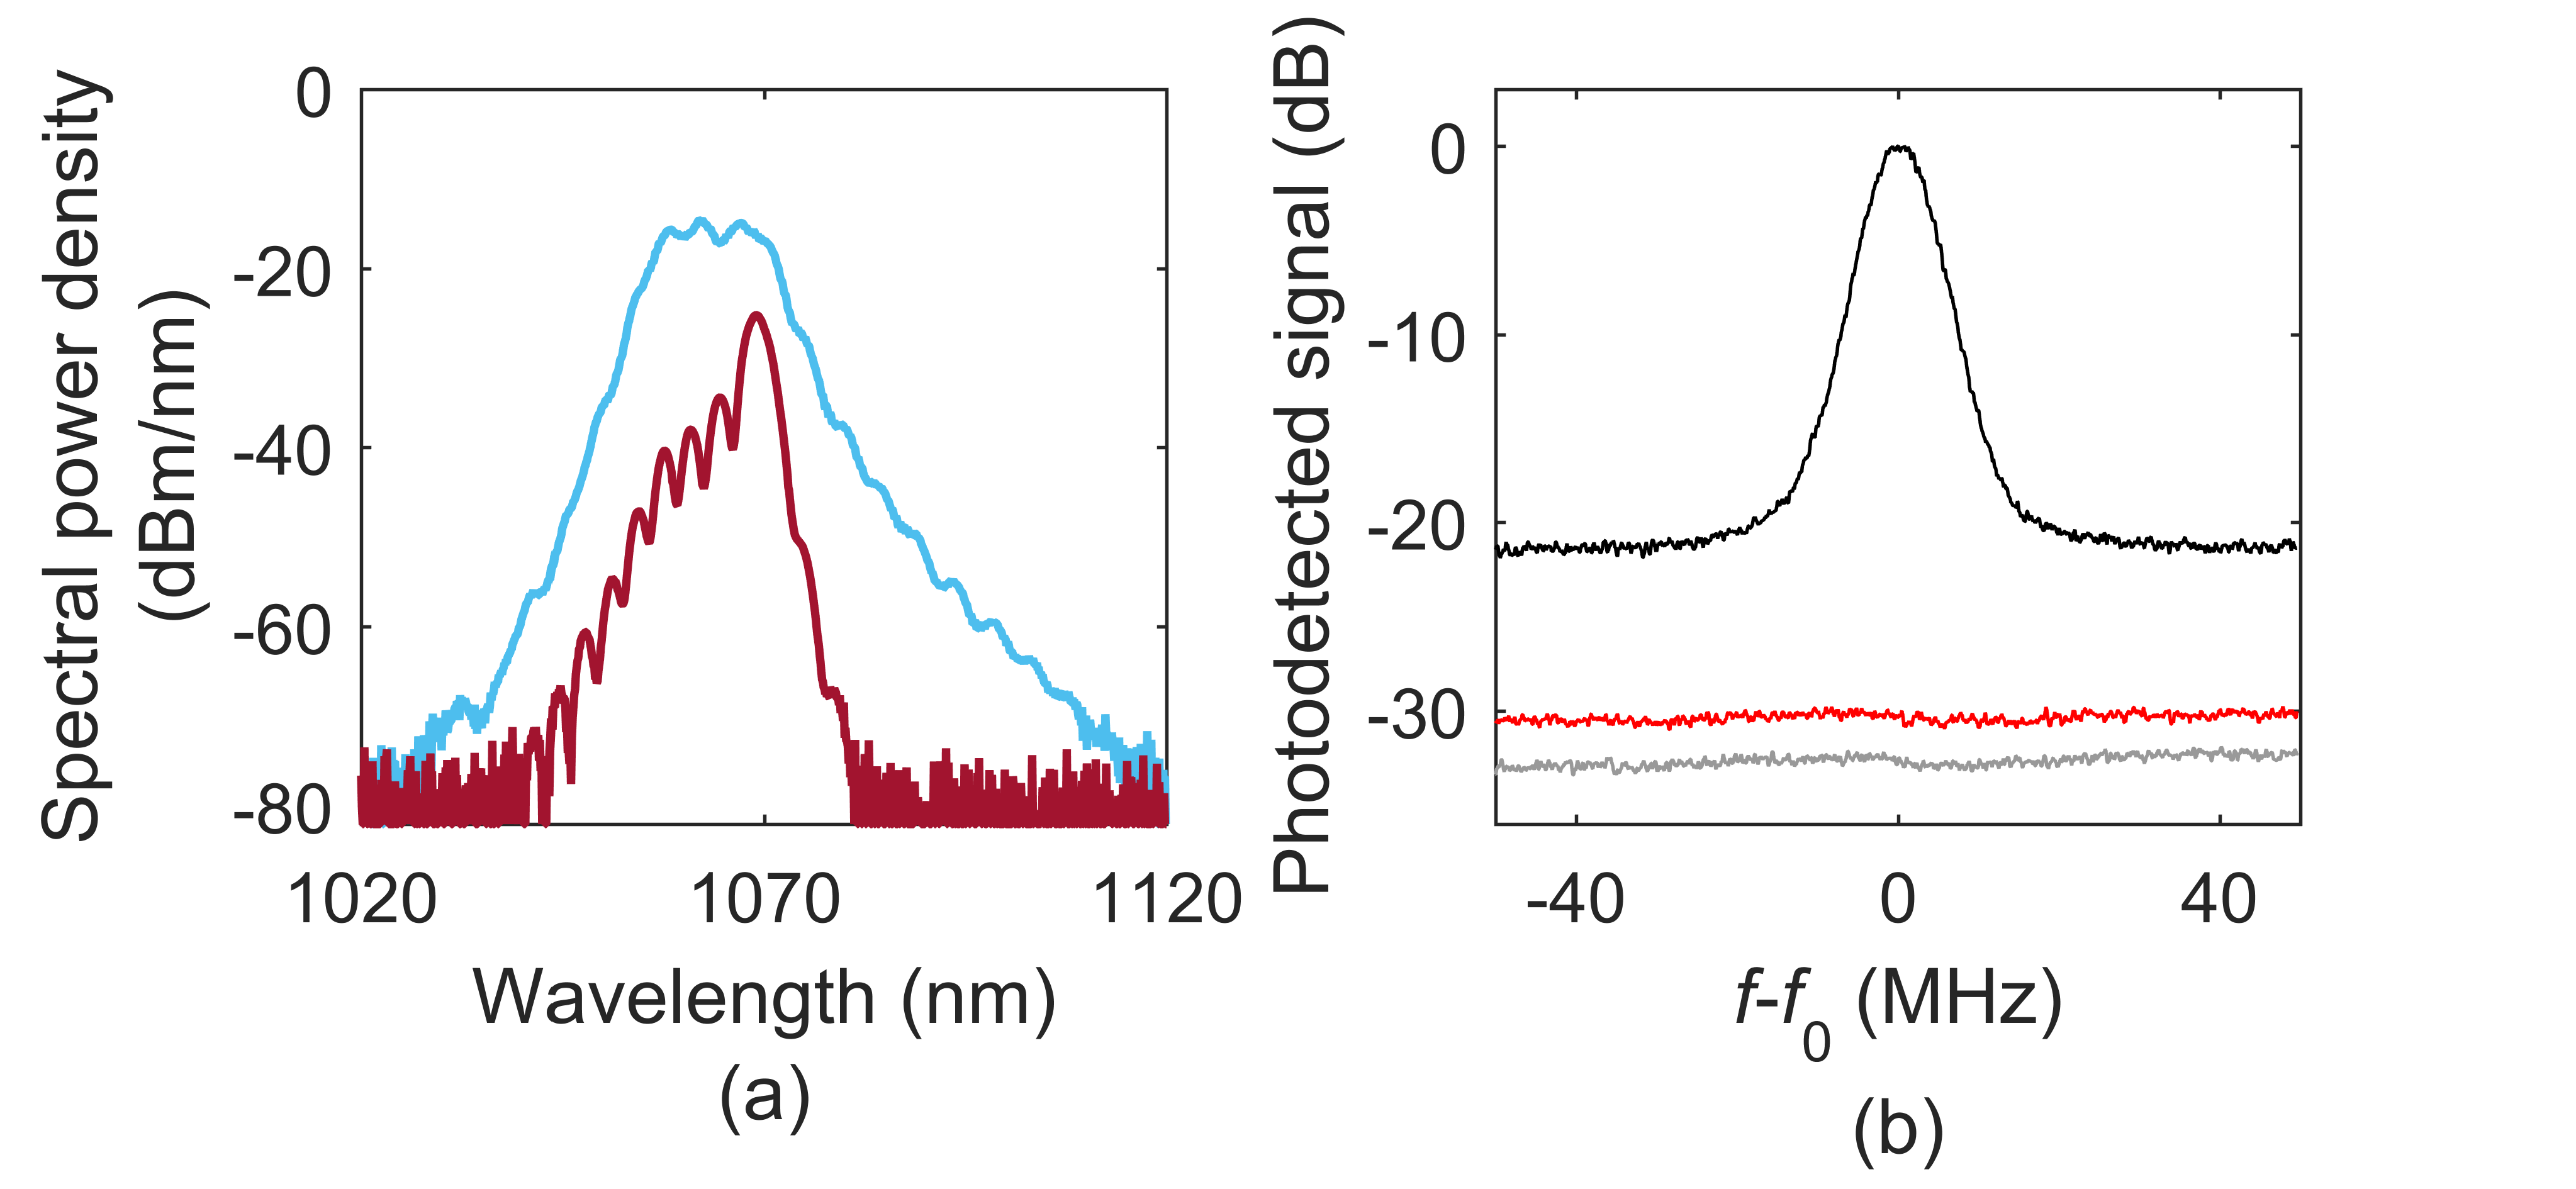
\includegraphics{\FigPath/Figures/EOMCombs/EOMCf0.png}
	\end{center}
	\caption[Self-referencing of an EOM comb]{\textbf{Self-referencing of an EOM comb.} (a) Spectral components used for $f-2f$ self-referencing after passing through a 1070-nm optical bandpass filter: native supercontinuum light (blue) and frequency-doubled 2140-nm supercontinuum light (red). (b) Photodetected carrier-envelope offset frequency signal (black), along with a measurement of the intensity noise of the pulse train and the photodetector noise floor (grey). The frequency of the detected signal is $f_0=706.6$ MHz.}
	\label{fig:EOMC_f0}
\end{figure} 



\section{Noise considerations in EOM comb generation}\label{sec:EOMCnoise}



The repetition rate of an EOM comb is derived from a microwave source and is multiplied directly by a factor $\mu$ to yield the frequency-comb mode with seed-laser-referenced mode number $\mu$. This is an important contrast with both modelocked-laser-based combs and microcombs, where generation of the comb in a resonant cavity dampens fast fluctuations of $f_{rep}$. In the EOM comb case, the contribution to the frequency noise of mode $\mu$ from the microwave source scales with $\mu$; the contribution to the power spectrum of frequency noise scales as $\mu^2$. This presents a challenge in the generation of the coherent octave-spanning supercontinuum spectrum required for $f-2f$ self-referencing, as the modes used for self-referencing are at the extreme ends of the supercontinuum where $\mu$ is large. The factor by which the noise on the modulation tone $f_{rep}$ is multiplied to determine its contribution to the noise on the measured carrier-envelope offset frequency is the ratio between the frequency $f_c$ of the seed laser and the repetition rate. It is easiest to see this by recalling that the carrier-envelope offset frequency, which is measured by $f-2f$ self-referencing, is $f_0=f_c-Nf_{rep}$, where $N$ is the largest integer such that $f_0>0$; therefore $\partial f_0/\partial f_{rep}=-N$. 

For the 10 GHz comb discussed above the noise on $f_{rep}$ contributes to the noise on $f_0$ after multiplication by a factor $N=f_c/f_{rep}\sim$19340 (where $f_c=$193.4 THz for a 1550 nm seed laser). In Fig. \ref{fig:EOMC_noise}a we plot this contribution to the spectrum of fluctuations the carrier-envelope offset frequency, as well as the contribution from the noise of the seed laser. The noise on $f_{rep}$ results from technical noise on the synthesizer tone at low Fourier frequencies and approaches a white Johnson-Nyquist (thermal) phase-noise floor of -177 dBm/Hz at high Fourier frequencies. Noise in each of these regimes impacts the photodetected $f_0$ signal: low-frequency noise contributes to the linewidth of the comb modes and therefore the $f_0$ signal, while high-frequency noise contributes to a frequency-noise floor on the photodetected signal \cite{DiDomenico2010}. Unmitigated multiplication of this thermal floor by the factor $N^2=$19340$^2$ leads to a supercontinuum with optical frequency fluctuations that are large enough to prevent detection and measurement of $f_0$; this is evidenced by unsuccessful attempts we have made to measure $f_0$ without the filter cavity in place.

\begin{figure}[htpb]
	\begin{center}
		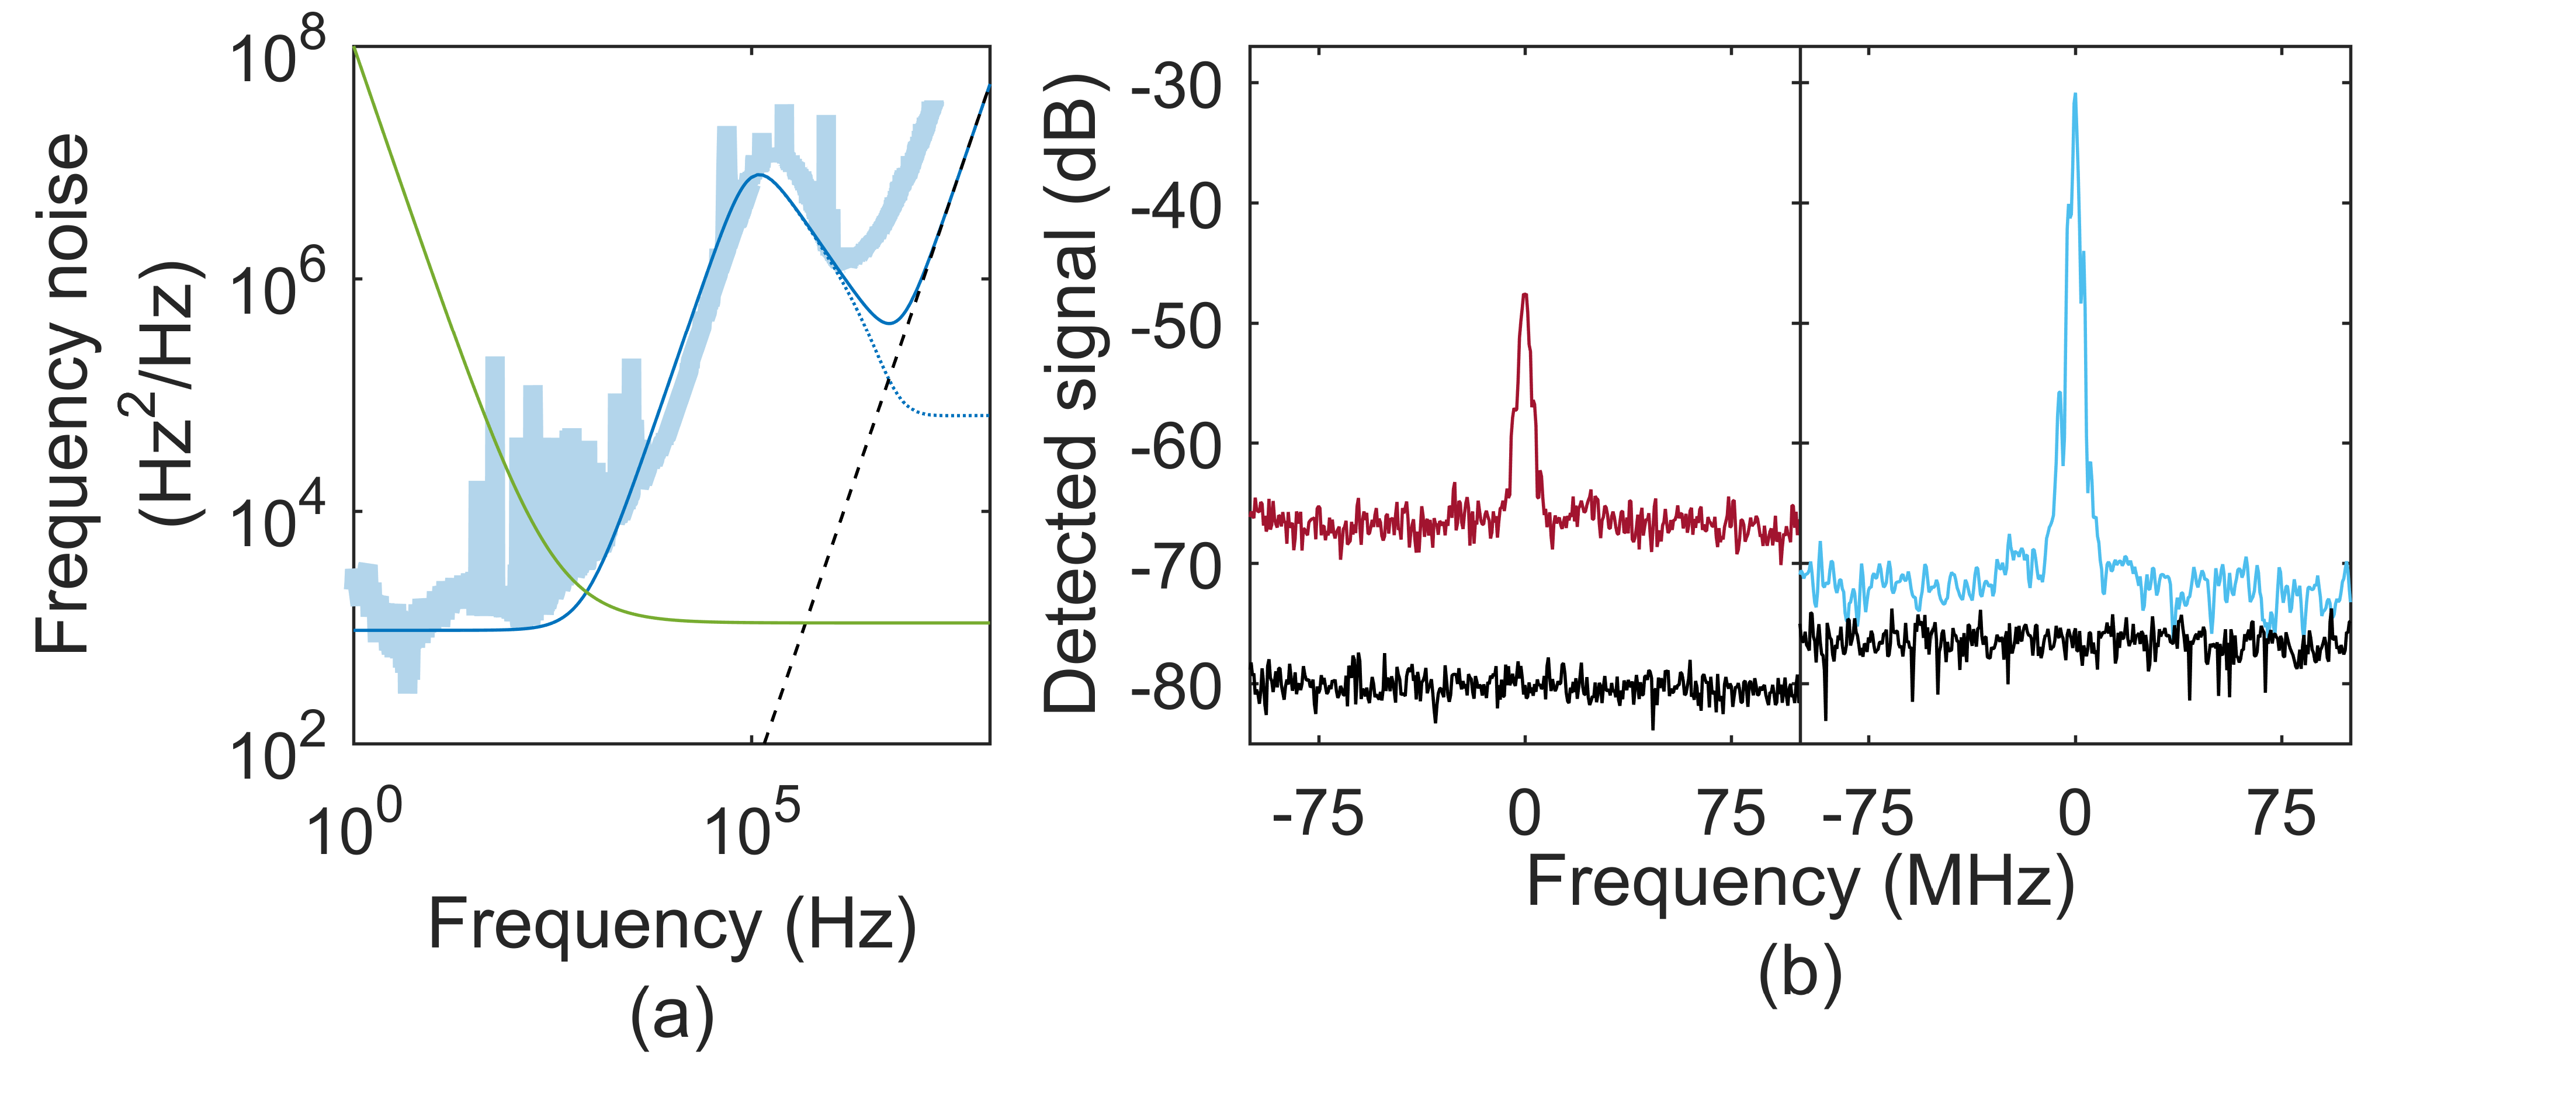
\includegraphics{\FigPath/Figures/EOMCombs/EOMCphasenoise.png}
	\end{center}
	\caption[Investigation of the noise properties of the EOM comb]{\textbf{Investigation of the noise properties of the EOM comb.}  (a) Contributions to the frequency-noise spectrum of the carrier-envelope offset frequency: model of the seed laser based on past measurements (green), model of the 10 GHz synthesizer multiplied by 19430$^2$ without the filter cavity (solid blue, measurement thick blue), and synthesizer multiplied by 19340$^2$ and the Lorentzian filter-cavity transfer function (dotted blue). The synthesizer is modeled at high frequency by noise increasing as $f^2$ (associated with a white phase-noise floor) that arises from Johnson-Nyquist noise with synthesizer power of -8 dBm. The thermal contribution alone is indicated by the dashed black line. (b) Comparison of the detected beats between the supercontinuum and a CW laser with 1319 nm wavelength without (red, left) and with (blue, right) the Fabry-Perot filter cavity. The level of intensity noise on the supercontinuum, measured by removing the 1319 nm CW laser, is shown by the lower gray trace in each plot; the elevated floor of the red trace relative to this background indicates that frequency noise is responsible for the reduced SNR of the beat without the filter cavity. Signal-to-noise ratios for the beat are 17 dB without and 40 dB with the filter cavity.}
	\label{fig:EOMC_noise}
\end{figure} 

Inclusion of the Fabry-Perot filter cavity in our system enables detection and measurement of $f_0$. We use a Fabry-Perot cavity with free-spectral range $\sim$10 GHz that is actively stabilized to the comb's mode spacing. Our filter cavity has linewidth 7.5 MHz; equivalently, it has finesse of $\mathcal{F}$=1333. The filter cavity's Lorentzian transfer function reduces the optical frequency fluctuations of the comb modes at high Fourier frequency---these fluctuations are averaged over the photon lifetime of the cavity. The effect of passing the comb through the cavity is demonstrated concretely in Fig. \ref{fig:EOMC_noise}b, where we compare the lineshape of a heterodyne beat between the supercontinuum and a CW laser with 1319 nm wavelength with and without the filter cavity in place. The signal-to-noise ratios for the beat with and without the filter cavity are 40 dB and 17 dB, respectively.




The filter cavity reduces the frequency noise of $f_0$ at Fourier frequencies outside of the cavity linewidth of 7.5 MHz. We explore the effect of fluctuations inside of the filter cavity's linewidth by changing the microwave source from which $f_{rep}$ is derived. The $f_0$ signal shown in Fig. \ref{fig:EOMC_f0}b is acquired with a tunable commercial synthesizer providing $f_{rep}$ after repetition-rate downsampling to 2.5 GHz. In Fig. \ref{fig:EOMC_f0_sources} we show the detected $f_0$ signal with three different sources for the 10 GHz repetition rate: 1. No downsampling, synthesizer at 10 GHz; 2. Dieletric-resonator oscillator; and 3. Sapphire oscillator. The $f_0$ beat without downsampling with $f_{rep}$ derived from the synthesizer has signal-to-noise ratio comparable to that of the $f_0$ beat measured at 2.5 GHz repetition rate, but with higher intensity noise on the supercontinuum due to uncontrolled differences in the nonlinear spectral broadening. The other two sources have significantly less noise at low Fourier frequencies, and the effect of this lower noise is readily apparent in the reduced linewidth of the $f_0$ signal. This indicates the importance of a high-performance microwave oscillator for future deployments of EOM combs. We emphasize that we have been unable to detect $f_0$ without the filter cavity, even with $f_{rep}$ derived from the sapphire oscillator. This is a confirmation that oscillator-independent thermal noise obscures $f_0$ without the filter cavity in place.



\begin{figure}[htpb]
	\begin{center}
		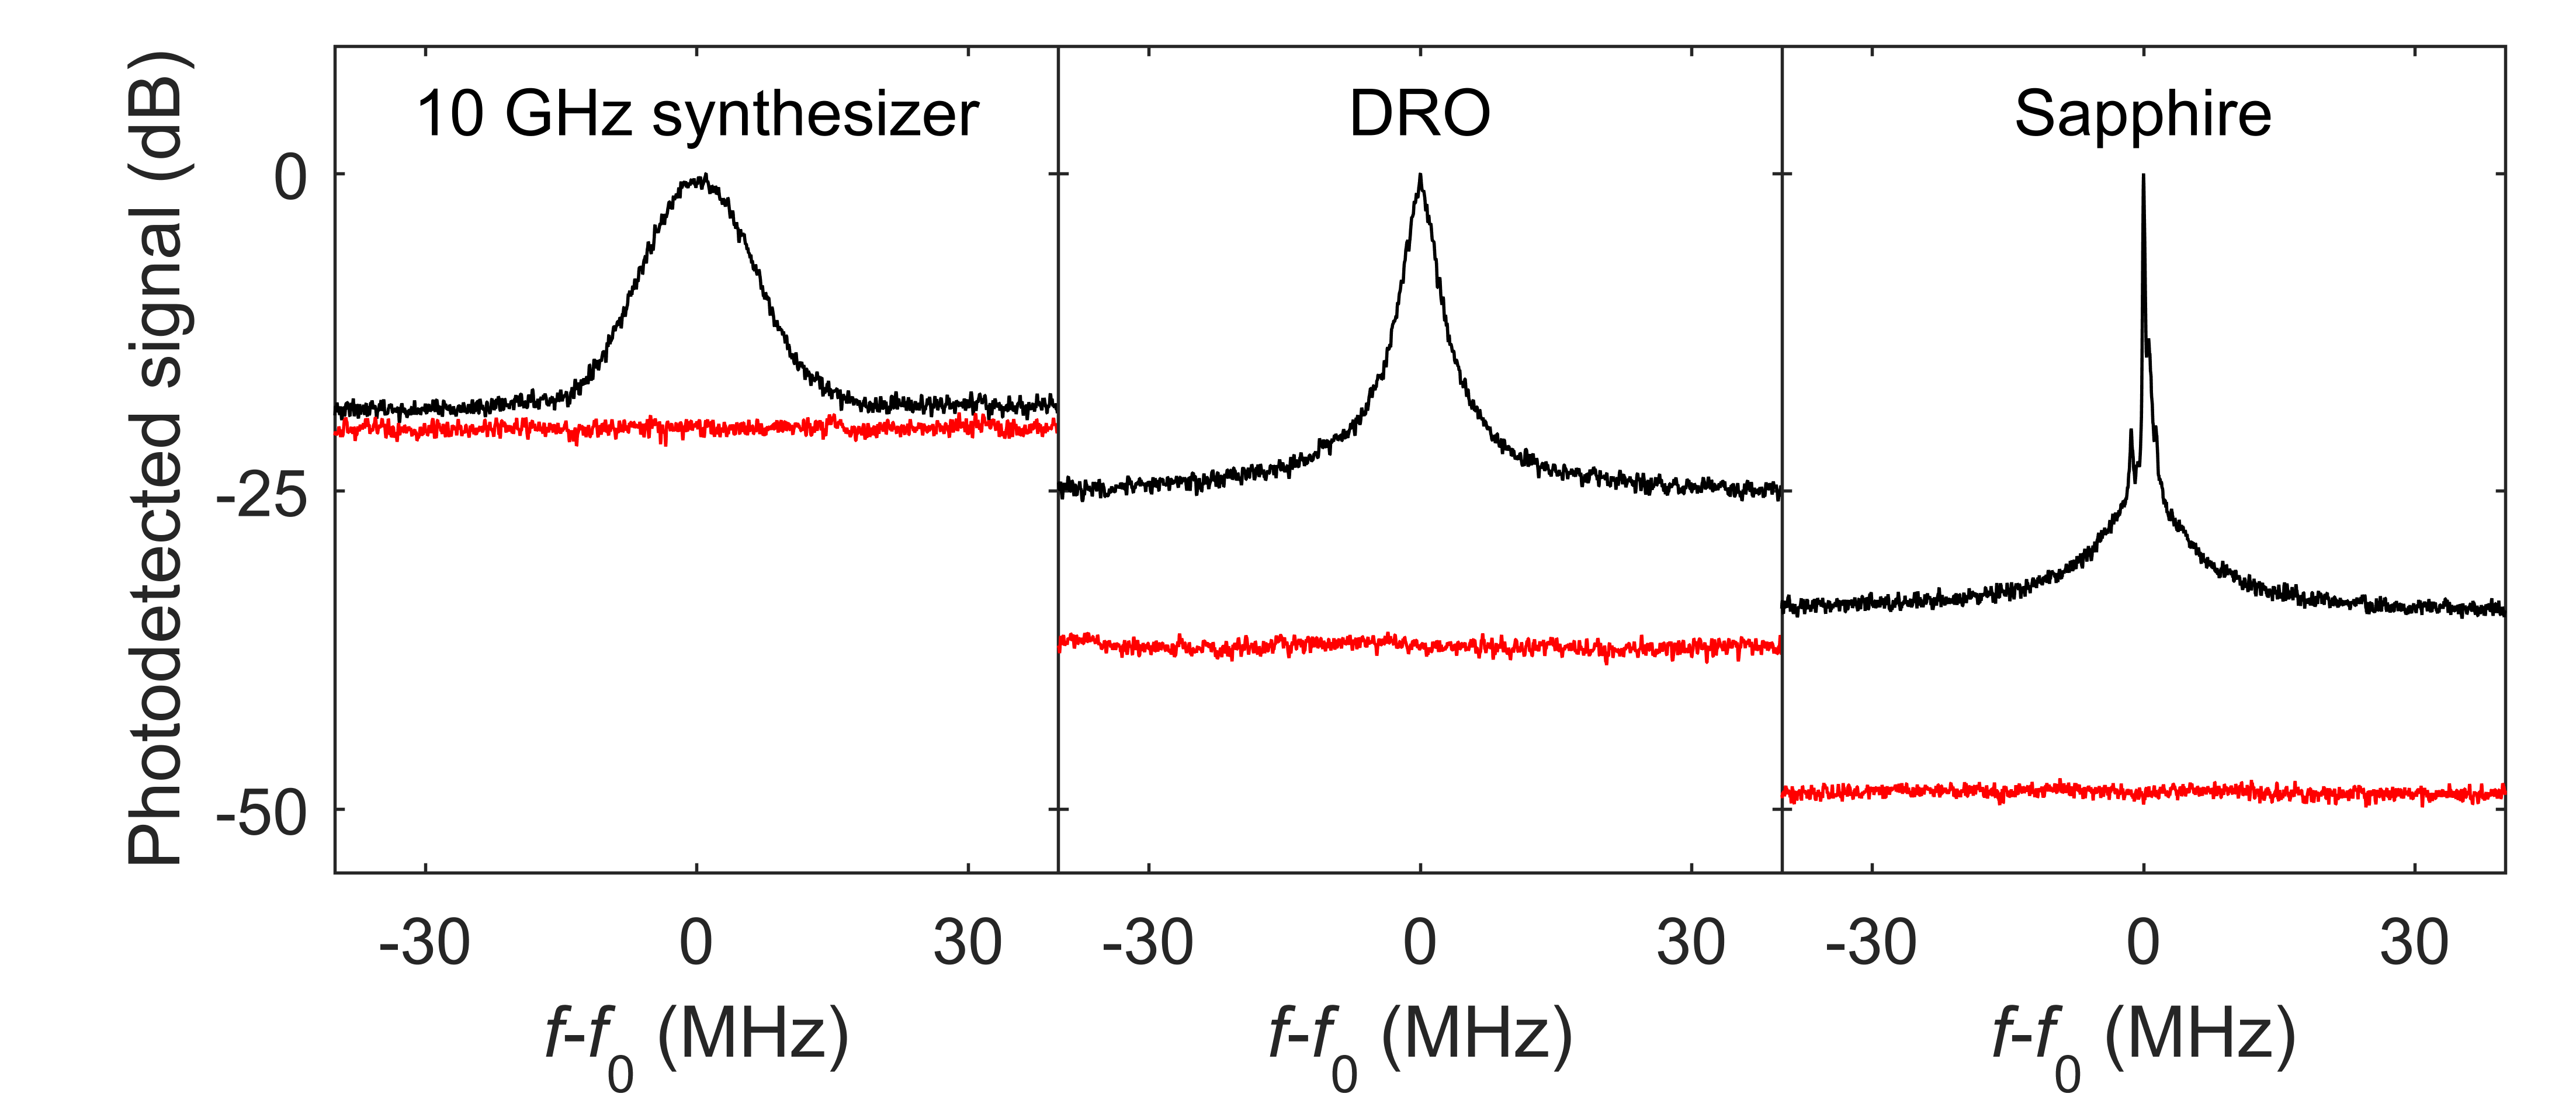
\includegraphics{\FigPath/Figures/EOMCombs/EOMCf0sources.png}
	\end{center}
	\caption[Photodetected carrier-envelope-offset frequency signal with different sources for $f_{rep}$]{\textbf{Photodetected carrier-envelope-offset frequency signal with different sources for $f_{rep}$.} (a) The $f_0$ beat with $f_{rep}$ derived from a synthesizer; $f_0=1.793$ GHz. (b) The same, with $f_{rep}$ derived from a dielectric-resonator oscillator; $f_0=491$ MHz. (b) The same, with $f_{rep}$ derived from a sapphire oscillator, $f_0=726$ MHz. Different $f_0$ linewidths for different $f_{rep}$ sources illustrate the effect of low-Fourier-frequency noise of $f_{rep}$ on the frequency-noise characteristics of the EOM comb.}
	\label{fig:EOMC_f0_sources}
\end{figure} 

\section{Application: Optical frequency division via double pinning}

\textit{Optical frequency division} (OFD) refers to the stabilization of a microwave frequency by locking it to a subharmonic of an optical frequency or frequency difference \cite{McFerran2005,Fortier2011}. This technique transfers the fractional frequency stability of the optical frequency to the microwave tone, and is a method for generation of stable microwaves that is competitive with all-electronic techniques. One method for OFD is to self-reference a frequency comb and lock $f_0$ to a microwave reference, and then lock the beat between the comb and a stable optical frequency $\nu_{opt}$ by feeding back to the repetition rate. An ideal lock transfers the noise on $\nu_{opt}$ to the repetition rate with a division factor $N$, where the beat is taken between $\nu_{opt}$ and mode $N$ with frequency $f_0+Nf_{rep}$. The repetition rate then acquires the fractional frequency stability of the optical reference.

A second method of performing OFD is \textit{double pinning}, in which the comb is not self-referenced, but instead two optical references are used to control the two comb degrees of freedom $f_{rep}$ and $f_0$ \cite{Swann2011,Papp2014,Li2014b}. As a demonstration of the utility of the EOM comb system, we perform OFD with double pinning using the EOM comb spectrum generated as described above.

\begin{figure}[htpb]
	\begin{center}
		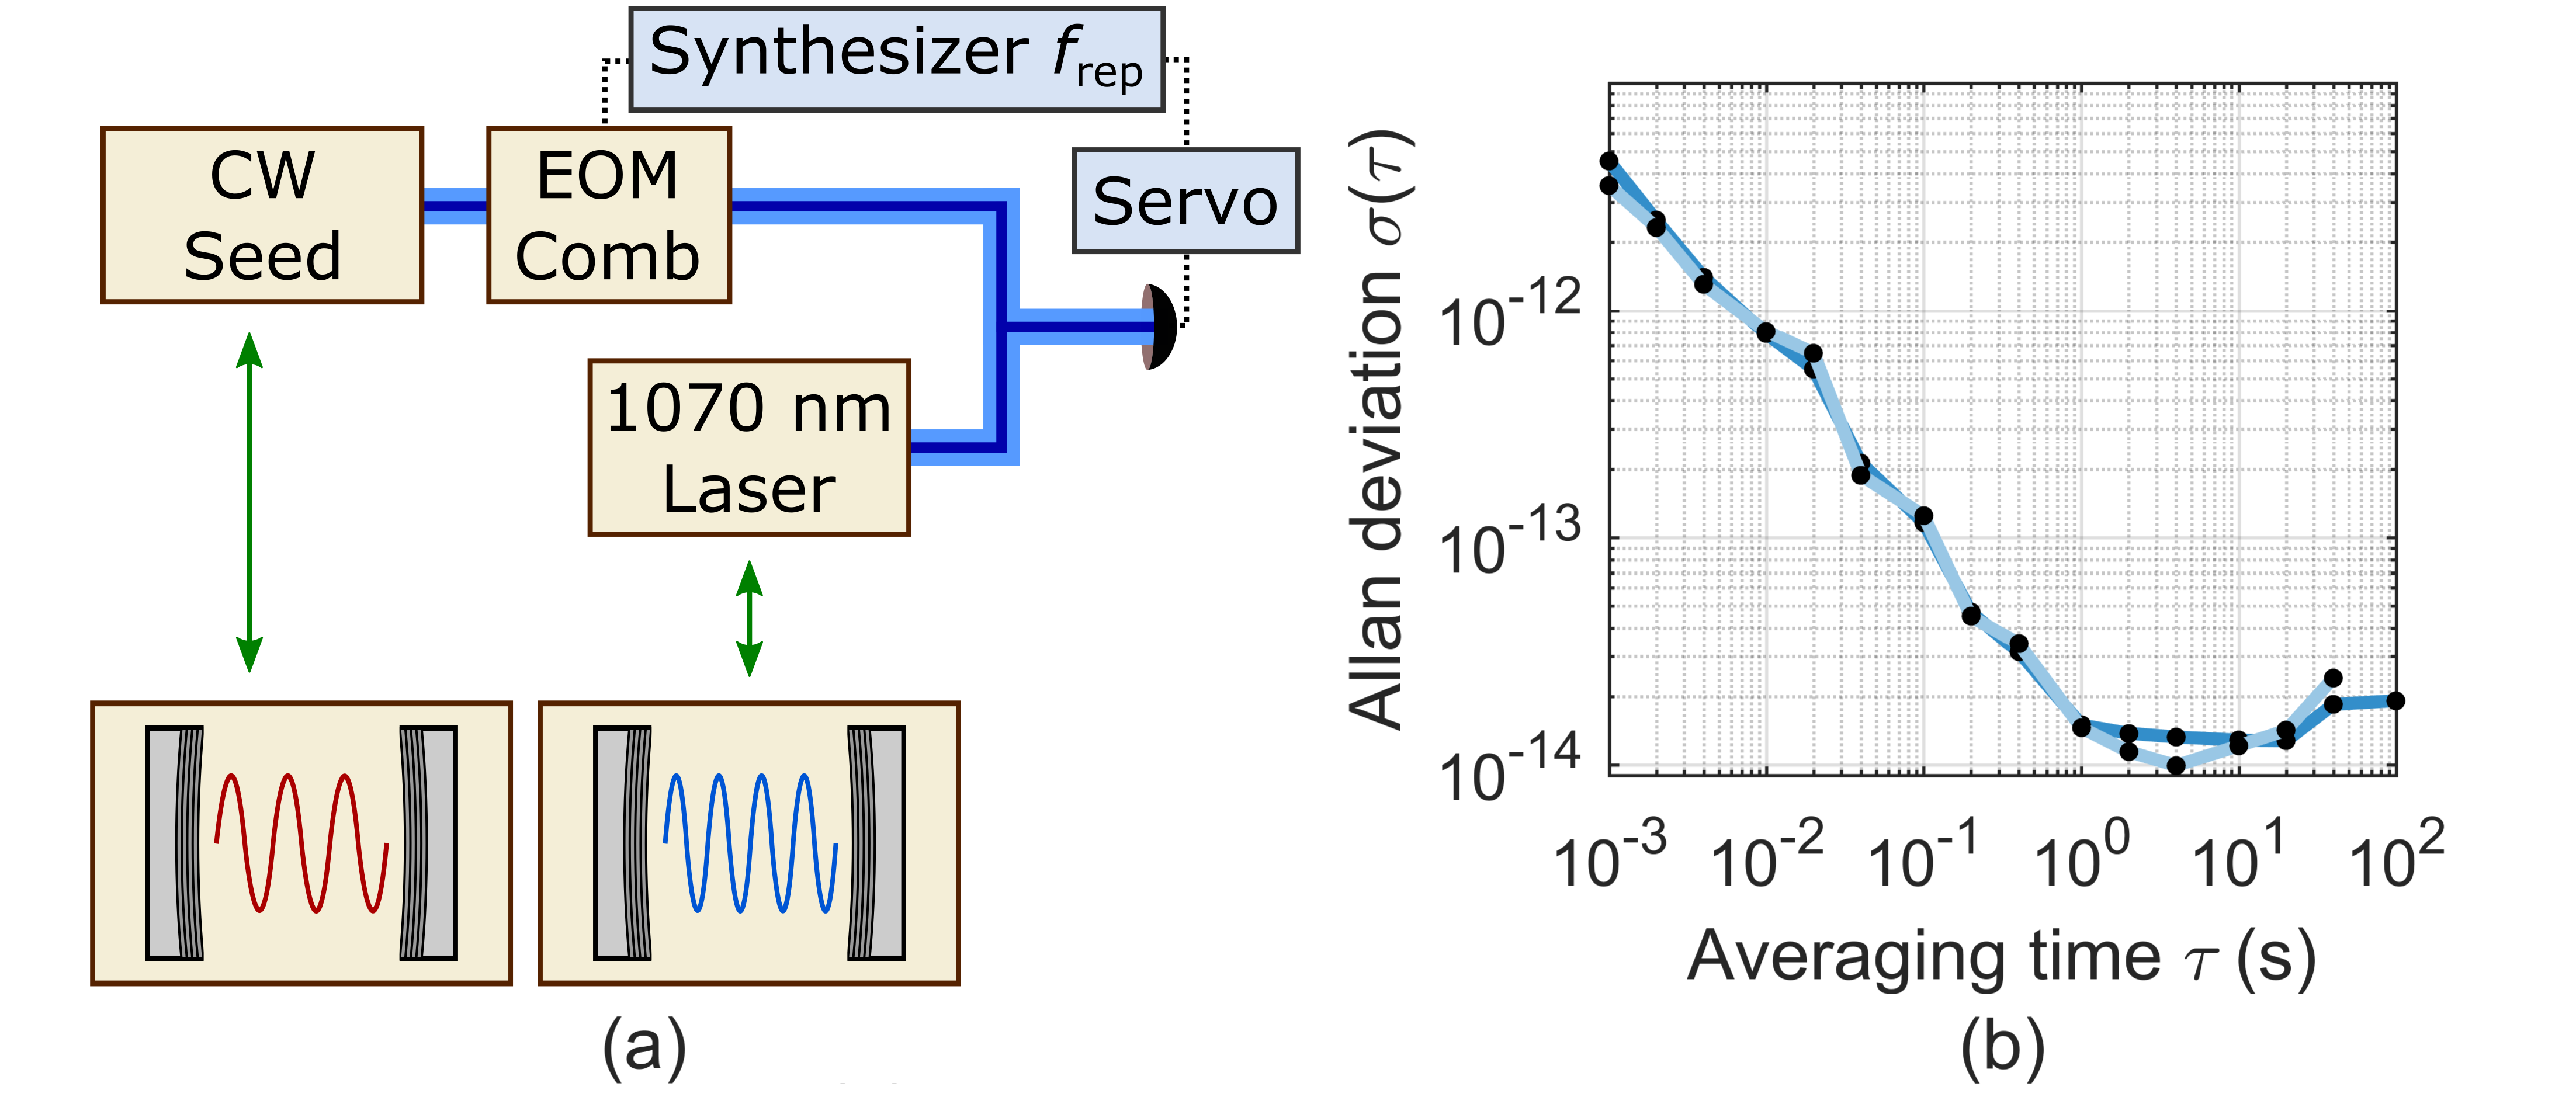
\includegraphics{\FigPath/Figures/EOMCombs/EOMCdoublepinning.png}
	\end{center}
	\caption[Stable microwave generation with an EOM comb via double pinning]{\textbf{Stable microwave generation with an EOM comb via double pinning.} (a) Experimental setup for double pinning of an EOM comb to two optical references. The seed laser for the EOM comb is locked to a stable reference cavity at 1550 nm, and a mode of the supercontinuum is locked to a second laser stabilized to a reference cavity at 1070 nm. The lock is achieved by feeding back to the synthesizer that generates $f_{rep}$. (b) Two measurements of the Allan deviation of the repetition rate of the double-pinned EOM comb. The Allan deviation at 1 s averaging time is $\sim1.5\times10^{-14}$, considerably better than what can be achieved by the synthesizer alone. At longer averaging times the frequency interval $f_{1070}-f_{1550}$ begins to change due to thermal drift, so the Allan deviation increases.}
	\label{fig:EOMCdoublepinning}
\end{figure} 

For our OFD experiment, we generate the EOM comb using a seed laser with frequency $f_{1550}$ that is locked to a stable reference cavity for 1550 nm wavelength. We also generate a second laser with frequency $f_{1070}$ that is stabilized to a reference cavity for 1070 nm wavelength. After generating the EOM comb supercontinuum, we measure the frequency of the beat between a mode of the EOM comb with pump-referenced mode number $\mu_b$ and frequency $f_{\mu b}=f_{1550}+\mu_b f_{rep}$ and the cavity-stabilized 1070 nm laser. We lock this beat to a microwave reference with frequency $f_{lock}$ by feeding back to the repetition rate of the EOM comb. This experimental setup is depicted schematically in Fig. \ref{fig:EOMCdoublepinning}a. The equation representing an ideal lock is:
\begin{equation}
0=f_{1550}+\mu_b f_{rep}-f_{1070}-f_{lock}.
\end{equation}
Then the fluctuations on the repetition rate are:
\begin{equation}
\delta f_{rep}=\delta(f_{1070}-f_{1550}+f_{lock})/\mu_b.
\end{equation}
Thus, the fluctuations on the repetition rate are the worse of (a) the absolute fluctuations on $f_b$ divided by $\mu_b$ and (b) the fractional fluctuations on $f_{1070}-f_{1550}$, since $f_{1070}-f_{1550}\sim\mu_b f_{rep}$.

We characterize the output of this OFD scheme by photodetecting the repetition rate of the OFD-stabilized EOM comb and measuring its Allan deviation $\sigma(\tau)$ \cite{Levine1999}. The Allan deviation is the square root of the Allan variance $\sigma^2(\tau)$, which is defined as:
\begin{equation}
\sigma^2(\tau)=\frac{1}{2}<(\overline{y}_{n+1}-\overline{y}_n)^2>.
\end{equation}
Here $<g>$ denotes the expectation value of $g$, which in practice is determined by recording many samples, and $\overline{y}_n$ is the $n$\textsuperscript{th} fractional frequency average, where each average is over a time $\tau$ and there is no dead time between them. The fractional frequency $y$ is defined relative to a nominal frequency $f_{nom}$: $y(t)=(f(t)-f_{nom})/f_{nom}$.

We measure the Allan deviation\footnote{This measurement is performed using a commercial characterization system that calculates the Allan deviation after counting and recording the input frequency signal. There are subtleties involved in measuring and calculating the Allan deviation, e.g. how to treat `dead time' between measurements, that are beyond the scope of this discussion \cite{Levine1999}---here we report the Allan deviation as recorded by the commercial system.} of $f_{rep}$ by measuring the difference between $f_{rep}$ and a reference 10 GHz signal that is derived through OFD with a Ti:sapphire modelocked laser \cite{Fortier2011}; the reference is known to have Allan deviation significantly lower than what we measure, so we know that the observed Allan deviation is not limited by the noise-floor of the measurement. We plot the result, $\sigma(\tau)$ as a function of averaging time $\tau$, for two separate measurements in Fig. \ref{fig:EOMCdoublepinning}b. The observed Allan deviation at one second averaging time $\sigma(\tau=$ 1 s$)\sim1.5\times10^{-14}$ is significantly better than the level $\sim10^{-13}$ that is achieved by the synthesizer alone, using just the hydrogen maser at NIST as a reference.



\section{Outlook}
The EOM comb approach for frequency-comb generation yields combs that are widely tunable and that can be flexibly tailored for specific applications. Because the comb generation is a non-resonant process (up to the optional inclusion of a filter cavity), the comb properties can be manipulated in real time with speed and range that greatly exceeds the capabilities of mode-locked lasers (where repetition-rate adjustment requires manipulation of moving parts) and microcombs (where repetition-rate control via phase modulation as described in Chap. \ref{chap:PMPumping}, for example, is limited to the locking range afforded by the resonator dispersion). This has allowed, for example, the recent proposal and demonstration of \textit{PHIRE}---Parallel Heterodyne Interferometry via Rep-rate Exchange---which is, essentially, dual-comb spectroscopy \cite{Coddington2016} with a single frequency comb whose repetition-rate is periodically switched \cite{Carlson2018}. 

EOM combs, with their lack of moving parts, also offer robust turn-key operation to a degree that is difficult to achieve with other comb sources. This has made them particularly promising for applications where long-term deployment with maximum up-time is important, such as calibration of astronomical spectrograms \cite{Metcalf2018}. While the necessity of the filter cavity described here to enable $f-2f$ self-referencing is an apparent limitation, there are promising routes towards eliminating this requirement---using a high-power, tunable microwave oscillator could allow self-referencing of a repetition-rate-tunable EOM comb without a filter cavity.

